\graphicspath{{Chapitre_2/Images/}}
\chapter{Introduction}\label{introduction}
\quad\, Since the end of the 17th century, people have started to study the conversion of the energy into a useful form. The purpose was to utilize the available raw energy to produce works.\\

Denis Papin, a french person borned in 1647 in the region of Chitenay, developed one of the first conversion machine in 1690. The machine, a steam piston engine, was powered by steam which produced a back and forth movement of the piston head generating power.

\begin{figure}[h]
    \centering
    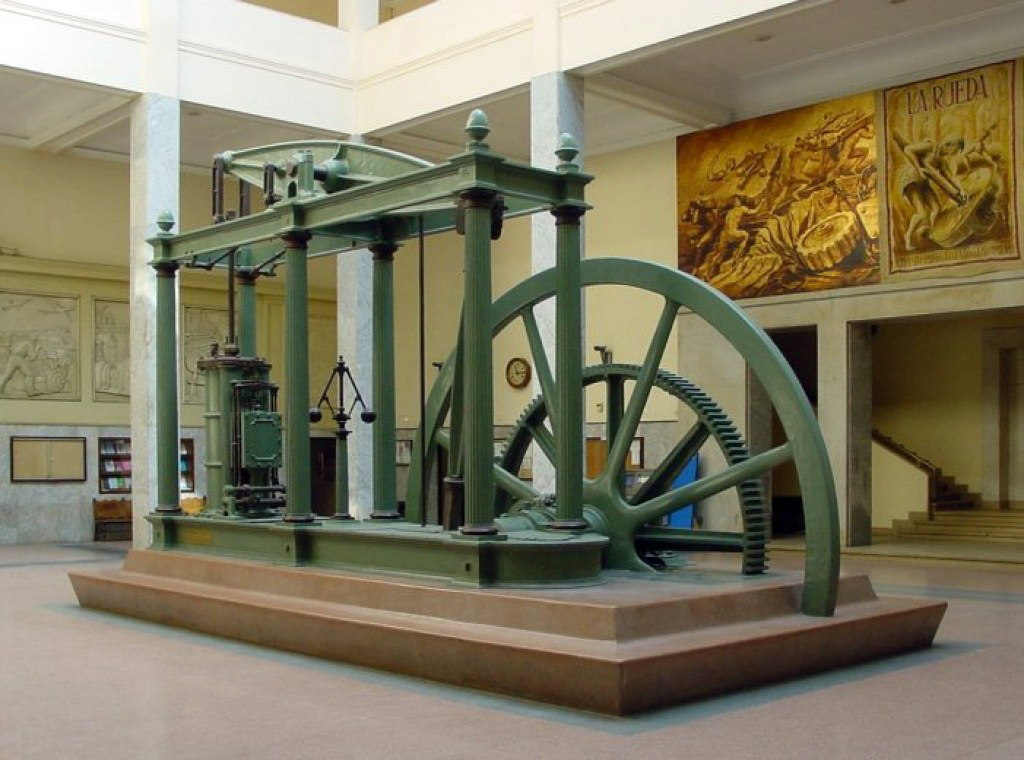
\includegraphics[width=0.6\textwidth]{Chapitre_1/Images/Maquina_vapor_Watt_ETSIIM.jpg}
    \caption{Watt steam machine\cite{Watt}}
    \label{fig:Watt}
\end{figure}

Then, later in the 18th, the British James Watt (1736 - 1819) invented and commercialized a steam machine. Thanks to the great marketing around his product, the machine (see Figure \ref{fig:Watt}), was very successful among the merchants. Indeed, it was sold as an alternative to horses and the capacity to produce works of the machine was express in horse power. 

James Watt named this quantifying unit the Watt unit (W), which will become later the standard unit for quantifying the power produced by a machine.\\

As a common knowledge, it is known that the steam machines have been an important element of the industrial revolution. The machines driven by wind and water have been progressively replaced by steam machines. It is only in the beginning of the 19th that this new technologies really started to be used. As examples, the applications were mining, merchandise transportation, etc...\\

In 1872, the American George Brayton (1830 - 1892) patented a gas internal combustion engine which was characterized by a continuous combustion \cite{Boles2006}. The  